\documentclass[aspectratio=169, table]{beamer}

\graphicspath{{../../images/}}
%\usepackage[beamertheme=./praditatheme]{Pradita}

\usepackage{listings}

\lstdefinelanguage{bash} {
	keywords={},
	basicstyle=\ttfamily\scriptsize,
	keywordstyle=\color{blue}\bfseries,
	ndkeywords={iex},
	ndkeywordstyle=\color{purple}\bfseries,
	sensitive=true,
	commentstyle=\color{gray},
	stringstyle=\color{red},
	numbers=left,
	numberstyle=\tiny\color{gray},
	breaklines=true,
	frame=lines,
	backgroundcolor=\color{lightgray!10},
	tabsize=2,
	comment=[l]{\#},
	morecomment=[s]{/*}{*/},
	commentstyle=\color{gray}\ttfamily,
	stringstyle=\color{purple}\ttfamily,
	showstringspaces=false
}


\lstdefinelanguage{docker} {
	keywords={FROM, EXPOSE, RUN, ARG, ENTRYPOINT, EXPOSE, WORKDIR, COPY, as}, 
	basicstyle=\ttfamily\scriptsize,
	keywordstyle=\color{blue}\bfseries,
	ndkeywords={iex},
	ndkeywordstyle=\color{purple}\bfseries,
	sensitive=true,
	commentstyle=\color{gray},
	stringstyle=\color{red},
	numbers=left,
	numberstyle=\tiny\color{gray},
	breaklines=true,
	frame=lines,
	backgroundcolor=\color{lightgray!10},
	tabsize=2,
	comment=[l]{\#},
	%	morecomment=[s]{}{},
	commentstyle=\color{gray}\ttfamily,
	stringstyle=\color{purple}\ttfamily,
	showstringspaces=false
}

\lstdefinelanguage{yaml} {
	keywords={ },
	basicstyle=\ttfamily\scriptsize,
	keywordstyle=\color{blue}\bfseries,
	ndkeywords={iex},
	ndkeywordstyle=\color{purple}\bfseries,
	sensitive=true,
	commentstyle=\color{gray},
	stringstyle=\color{red},
	numbers=left,
	numberstyle=\tiny\color{gray},
	breaklines=true,
	frame=lines,
	backgroundcolor=\color{lightgray!10},
	tabsize=2,
	comment=[l]{\#},
	%	morecomment=[s]{}{},
	commentstyle=\color{gray}\ttfamily,
	stringstyle=\color{purple}\ttfamily,
	showstringspaces=false
}

\usetheme{Pradita}
\title{\LARGE{Chapter-02:}\\ \Huge{Container} \vspace{20pt}}
\subtitle{IF231303-Software Architecture}
\author{Alfa yohannis}
\begin{document}

    \begin{frame}[plain]
        \maketitle
    \end{frame}

    \begin{frame}
        \frametitle{What are Containers?}
        \begin{itemize}
            \item Containers are lightweight, stand-alone, executable packages that include everything needed to run a piece of software: code, runtime, system tools, libraries, and settings.
            \item They share the operating system kernel and isolate application processes from the host system and each other.
        \end{itemize}
    \end{frame}

    \begin{frame}
        \frametitle{Understanding Docker}
        \begin{itemize}
            \item Docker is a popular platform for developing, shipping, and running applications using containerization.
            \item It enables you to separate your applications from your infrastructure to deliver software quickly and reliably.
            \item Docker provides the ability to package and run an application in a loosely isolated environment called a container.
        \end{itemize}
    \end{frame}


    \begin{frame}
        \frametitle{Background and Motivation}
        \begin{itemize}
            \item \textbf{Traditional Virtualization:} Heavyweight, slower, and more resource-intensive.
            \item \textbf{Containers:} Lightweight, fast, share the host OS kernel, and require fewer resources.
            \item Need for a consistent development environment to avoid "works on my machine" issues.
            \item Facilitates microservices architecture, allowing easy deployment and scaling of applications.
        \end{itemize}
    \end{frame}


    \begin{frame}{Container vs Virtual Machine}
        \vspace{30pt}
        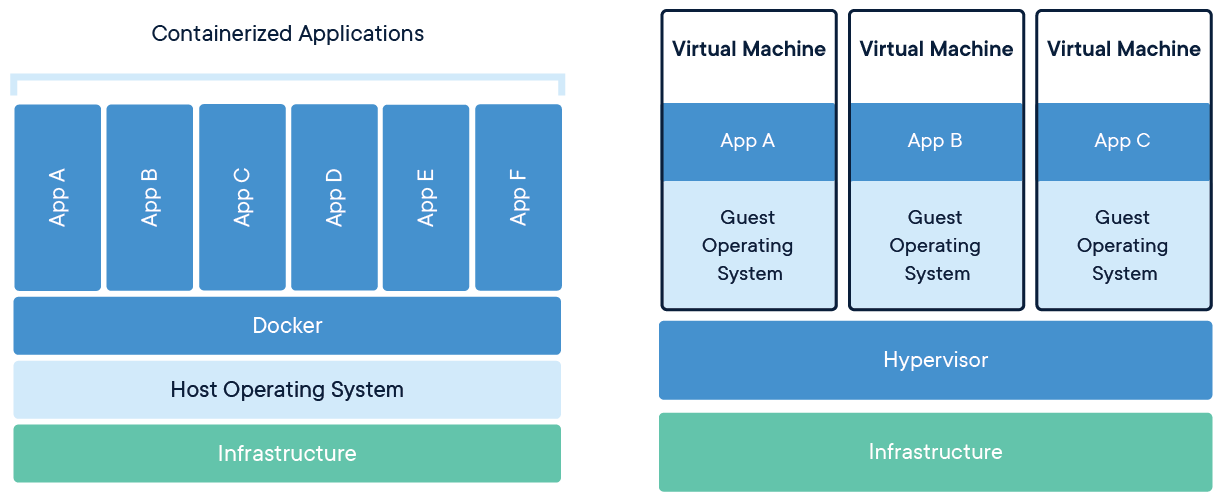
\includegraphics[width=\textwidth]{../../images/container-vm.png}
    \end{frame}


    \begin{frame}
        \frametitle{Container vs Virtual Machine}
        \vspace{25pt}
        \begin{itemize}
            \item \textbf{Virtual Machines:}
            \begin{itemize}
                \item Include the entire OS.
                \item Heavyweight and require more resources.
                \item Slower to start up.
                \item \textbf{Hypervisor:} Manages virtual machines, allowing multiple VMs to run on a single physical machine by abstracting hardware resources.
            \end{itemize}
            \item \textbf{Containers:}
            \begin{itemize}
                \item Share the host OS kernel.
                \item Lightweight and require fewer resources.
                \item Faster to start up.
            \end{itemize}
            \item Containers are ideal for microservices and DevOps practices due to their efficiency and scalability.
        \end{itemize}
    \end{frame}

     %        \framesubtitle{}
    \begin{frame}{Docker}
        \vspace{30pt}
        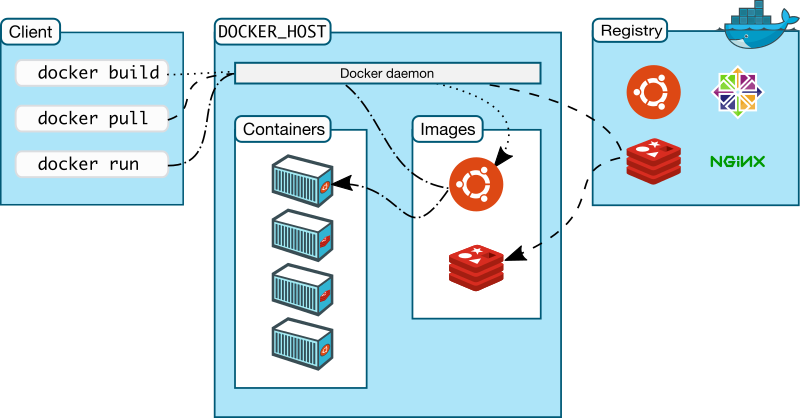
\includegraphics[width=\textwidth]{../../images/docker.png}
    \end{frame}

    \begin{frame}
        \frametitle{Components}
        \begin{itemize}
            \item \textbf{Docker Engine:} The core part of Docker, consisting of:
            \begin{itemize}
                \item \textbf{Docker Daemon:} Runs on the host machine and manages Docker containers, images, networks, and storage volumes.
                \item \textbf{Docker Client:} The command-line interface that users interact with.
            \end{itemize}
            \item \textbf{Images:} Read-only templates used to create containers.
            \item \textbf{Containers:} Runnable instances of Docker images.
            \item \textbf{Docker Registry:} Stores Docker images (e.g., Docker Hub).
        \end{itemize}
    \end{frame}

    \begin{frame}
        \frametitle{Advantages of Using Containers}
        \begin{itemize}
            \item \textbf{Portability:} Consistent environments across different platforms.
            \item \textbf{Efficiency:} Reduced overhead compared to virtual machines.
            \item \textbf{Scalability:} Easily scale up or down based on demand.
            \item \textbf{Isolation:} Applications run in isolated environments, preventing conflicts.
            \item \textbf{CI/CD:} Streamlines the process of development, testing, and deployment.
        \end{itemize}
    \end{frame}


    \begin{frame}
        \frametitle{Drawbacks of Containers}
        \begin{itemize}
            \item \textbf{Security:} Shared kernel can pose a security risk.
            \item \textbf{Persistence:} Managing stateful applications can be challenging.
            \item \textbf{Networking:} Complex networking setups can be difficult to manage.
            \item \textbf{Compatibility:} Not all applications are suited for containerization.
        \end{itemize}
    \end{frame}


    \begin{frame}
        \frametitle{Examples of Applications}
        \begin{itemize}
            \item \textbf{Web Applications:} Deploy web services with consistent environments.
            \item \textbf{Microservices:} Implement microservices architecture with isolated services.
            \item \textbf{Development Environments:} Create consistent development and testing environments.
            \item \textbf{Data Processing:} Run data processing tasks in isolated containers.
            \item \textbf{CI/CD Pipelines:} Automate the build, test, and deployment processes.
        \end{itemize}
    \end{frame}


    \begin{frame}
        \frametitle{Conclusions}
        \begin{itemize}
            \item Containers, especially with Docker, revolutionize software development and deployment.
            \item They provide lightweight, consistent, and isolated environments.
            \item While there are challenges, the benefits often outweigh the drawbacks, particularly in scalable and microservice-based architectures.
        \end{itemize}
    \end{frame}

\begin{frame}{Example: Employee Performance}
	\vspace{10pt}
	\begin{figure}
		\centering
		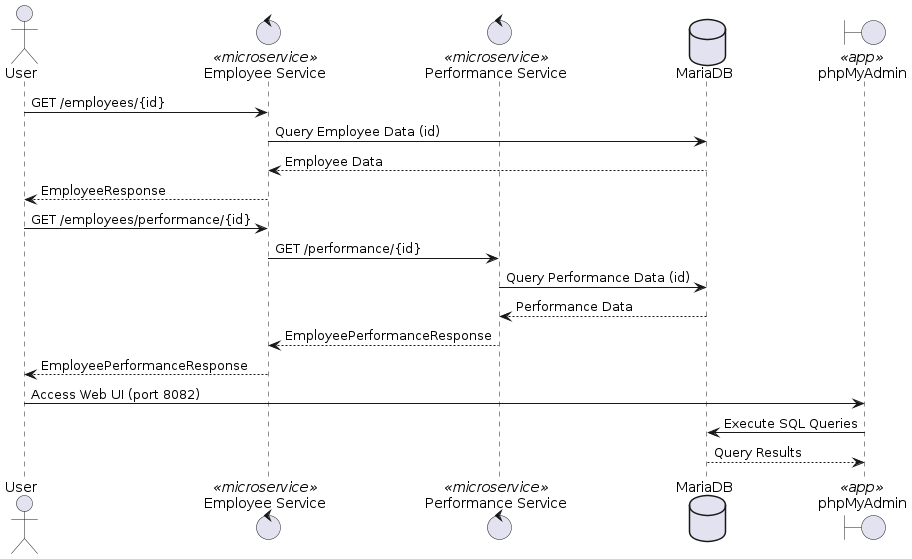
\includegraphics[width=0.8\textwidth]{../../images/out/microservices-employees.png}
		\label{fig:employee_performance}
	\end{figure}
\end{frame}

\begin{frame}{Instalasi dan Pengecekan Docker}
	Untuk menjalankan sistem berbasis \textit{container Docker}, langkah pertama adalah memastikan Docker telah terinstal dan berjalan dengan baik di sistem.
	
	\textbf{Langkah-langkah:}
	\begin{itemize}
		\item Instalasi Docker di berbagai sistem operasi.
		\item Verifikasi apakah Docker telah terinstal.
		\item Mengecek status Docker.
		\item Menjalankan container uji coba.
	\end{itemize}
\end{frame}

\begin{frame}[fragile]{Instalasi Docker}
	\textbf{1. Unduh dan Instal Docker} \\
	\begin{itemize}
		\item \textbf{Linux (Ubuntu/Debian)}:
		\begin{lstlisting}[language=bash]
			sudo apt update
			sudo apt install docker.io -y
			sudo systemctl enable --now docker
		\end{lstlisting}
		\item \textbf{Windows/macOS}: \\
		Kunjungi \texttt{https://www.docker.com/get-started}, unduh dan instal Docker Desktop.
	\end{itemize}
	
	\textbf{2. Verifikasi Instalasi Docker} \\
	\begin{lstlisting}[language=bash]
		docker --version
	\end{lstlisting}
	Jika berhasil, perintah ini akan menampilkan versi Docker yang terpasang.
\end{frame}

\begin{frame}[fragile]{Mengecek dan Menjalankan Docker}
	\textbf{1. Mengecek Status Docker} \\
	\begin{lstlisting}[language=bash]
		sudo systemctl status docker
	\end{lstlisting}
	Jika Docker tidak aktif, jalankan:
	\begin{lstlisting}[language=bash]
		sudo systemctl start docker
	\end{lstlisting}
	
	\textbf{2. Menjalankan Container Uji Coba} \\
	\begin{lstlisting}[language=bash]
		docker run hello-world
	\end{lstlisting}
	Jika berjalan dengan baik, pesan konfirmasi akan ditampilkan.
\end{frame}

\begin{frame}[fragile]{Instalasi dan Pengecekan Docker Compose}
	\textit{Docker Compose} digunakan untuk mengelola beberapa container Docker sebagai satu kesatuan dalam sebuah aplikasi. 
	
	\textbf{Langkah-langkah:}
	\begin{itemize}
		\item Instalasi Docker Compose di berbagai sistem operasi.
		\item Verifikasi apakah Docker Compose telah terinstal.
		\item Mengecek dan menjalankan layanan dengan Docker Compose.
	\end{itemize}
\end{frame}

\begin{frame}[fragile]{Instalasi Docker Compose}
	\vspace{20pt}
	\textbf{1. Unduh dan Instal Docker Compose} \\
	\begin{itemize}
		\item \textbf{Linux (Ubuntu/Debian)}:
		\begin{lstlisting}[language=bash]
			sudo apt update
			sudo apt install docker-compose -y
		\end{lstlisting}
		\item \textbf{Windows/macOS}: \\
		Docker Compose sudah termasuk dalam Docker Desktop. Kunjungi \texttt{https://www.docker.com/get-started} dan pastikan Docker Desktop telah terinstal.
	\end{itemize}
	
	\textbf{2. Verifikasi Instalasi Docker Compose} \\
	\begin{lstlisting}[language=bash]
		docker-compose --version
	\end{lstlisting}
	Jika instalasi berhasil, akan menampilkan versi Docker Compose yang terpasang.
\end{frame}

\begin{frame}[fragile]{Mengecek dan Menjalankan Docker Compose}
	\vspace{20pt}
	\textbf{1. Menjalankan Layanan dengan Docker Compose} \\
	Jalankan perintah berikut untuk memulai semua layanan:
	\begin{lstlisting}[language=bash]
		docker-compose up -d
	\end{lstlisting}
	\begin{itemize}
		\item Semua container dalam \texttt{docker-compose.yml} akan dijalankan.
		\item Mode \texttt{-d} membuatnya berjalan di latar belakang.
	\end{itemize}
	
	\textbf{2. Mengecek Status Container}. Menampilkan daftar container yang sedang berjalan. \\
	\begin{lstlisting}[language=bash]
		docker-compose ps
	\end{lstlisting}
	
	\textbf{3. Menghentikan Semua Container}. Perintah ini akan menghentikan dan menghapus semua container yang berjalan. \\
	\begin{lstlisting}[language=bash]
		docker-compose down
	\end{lstlisting}
\end{frame}

\begin{frame}[fragile]{Dockerfile untuk Performance Service}
	\vspace{20pt}
	Berikut adalah \texttt{Dockerfile} yang digunakan untuk membangun dan menjalankan \textit{Performance Service} menggunakan pendekatan \textit{multi-stage build}:
	
	\begin{lstlisting}[language=docker]
		# STEP 1
		FROM maven:3.9.6-eclipse-temurin-17 as build
		
		WORKDIR /workspace/app
		
		COPY pom.xml .
		COPY src src
		
		RUN mvn install -DskipTests
		RUN mkdir -p target/dependency && (cd target/dependency; jar -xf ../*.jar)
		
		COPY application.properties target/dependency
	\end{lstlisting}
\end{frame}

\begin{frame}[fragile]{Tahap Runtime dalam Dockerfile}
		\vspace{20pt}
	Setelah tahap build selesai, berikut adalah bagian Dockerfile yang menyiapkan lingkungan runtime untuk menjalankan aplikasi:
	
	\begin{lstlisting}[language=docker]
		# STEP 2
		FROM maven:3.9.6-eclipse-temurin-17
		EXPOSE 8081
		#VOLUME /tmp
		ARG DEPENDENCY=/workspace/app/target/dependency
		COPY --from=build ${DEPENDENCY}/BOOT-INF/lib /app/lib
		COPY --from=build ${DEPENDENCY}/META-INF /app/META-INF
		COPY --from=build ${DEPENDENCY}/BOOT-INF/classes /app
		COPY --from=build ${DEPENDENCY}/BOOT-INF/classes /app
		COPY --from=build ${DEPENDENCY}/application.properties /app
		ENTRYPOINT ["java","-cp","app:app/lib/*","software.architecture.microservice.PerformanceServiceApplication"]
	\end{lstlisting}
\end{frame}


\begin{frame}[fragile]{Dockerfile untuk Employee Service}
	\vspace{20pt}
	Berikut adalah \texttt{Dockerfile} yang digunakan untuk membangun dan menjalankan \textit{Employee Service} menggunakan pendekatan \textit{multi-stage build}:
	
	\begin{lstlisting}[language=docker]
		FROM maven:3.9.6-eclipse-temurin-17 as build
		
		WORKDIR /workspace/app
		
		COPY pom.xml .
		COPY src src
		
		RUN mvn install -DskipTests
		RUN mkdir -p target/dependency && (cd target/dependency; jar -xf ../*.jar)
		
		COPY application.properties target/dependency
	\end{lstlisting}
\end{frame}

\begin{frame}[fragile]{Tahap Runtime dalam Dockerfile}
	\vspace{20pt}
	Setelah tahap build selesai, berikut adalah bagian Dockerfile yang menyiapkan lingkungan runtime untuk menjalankan aplikasi:
	
	\begin{lstlisting}[language=docker]
		FROM maven:3.9.6-eclipse-temurin-17
		EXPOSE 8080
		#VOLUME /tmp
		ARG DEPENDENCY=/workspace/app/target/dependency
		COPY --from=build ${DEPENDENCY}/BOOT-INF/lib /app/lib
		COPY --from=build ${DEPENDENCY}/META-INF /app/META-INF
		COPY --from=build ${DEPENDENCY}/BOOT-INF/classes /app
		COPY --from=build ${DEPENDENCY}/BOOT-INF/classes /app
		COPY --from=build ${DEPENDENCY}/application.properties /app
		ENTRYPOINT ["java","-cp","app:app/lib/*","software.architecture.microservice.EmployeeServiceApplication"]
	\end{lstlisting}
\end{frame}


\begin{frame}[fragile]{Konfigurasi Jaringan Docker Compose}
	\vspace{20pt}
	\begin{columns}
		\column{0.55\textwidth}
		\begin{lstlisting}[language=yaml]
			networks:
				microservices:
				name: microservices
				driver: bridge
		\end{lstlisting}
		
		\column{0.45\textwidth}
		\textbf{Penjelasan:}
		\begin{itemize}
			\item Jaringan \texttt{microservices} digunakan untuk komunikasi antar container.
			\item \texttt{bridge} memungkinkan layanan Docker untuk berkomunikasi dalam satu jaringan internal.
		\end{itemize}
	\end{columns}
\end{frame}

\begin{frame}[fragile]{Konfigurasi Database: MariaDB}
	\vspace{20pt}
	\begin{columns}
		\column{0.55\textwidth}
		\begin{lstlisting}[language=yaml]
			services:
				mariadb:
				image: mariadb:latest
				container_name: mariadb
				environment:
				- MYSQL_ROOT_PASSWORD=1234
				- MYSQL_USER=alfa
				- MYSQL_PASSWORD=1234
				ports:
				- "3306:3306"
				restart: always
				networks:
				microservices:
				aliases:
				- mariadb
		\end{lstlisting}
		
		\column{0.45\textwidth}
		\textbf{Penjelasan:}
		\begin{itemize}
			\item Menggunakan image \texttt{mariadb:latest}.
			\item Variabel lingkungan mengatur kredensial database.
			\item Terhubung ke jaringan \texttt{microservices} dengan alias \texttt{mariadb}.
		\end{itemize}
	\end{columns}
\end{frame}

\begin{frame}[fragile]{Konfigurasi phpMyAdmin}
	\vspace{20pt}
	\begin{columns}
		\column{0.55\textwidth}
		\begin{lstlisting}[language=yaml]
			phpmyadmin:
				image: phpmyadmin/phpmyadmin:latest
				container_name: phpmyadmin
				ports:
				- "8082:80"
				restart: always
				depends_on:
				- mariadb
				environment:
				PMA_HOST: mariadb
				PMA_PORT: 3306
				networks:
				microservices:
				aliases:
				- phpmyadmin
		\end{lstlisting}
		
		\column{0.45\textwidth}
		\textbf{Penjelasan:}
		\begin{itemize}
			\item Layanan phpMyAdmin untuk mengelola database MariaDB.
			\item Dapat diakses di port \texttt{8082}.
			\item \texttt{depends\_on} memastikan MariaDB berjalan terlebih dahulu.
		\end{itemize}
	\end{columns}
\end{frame}

\begin{frame}[fragile]{Konfigurasi Performance Service}
	\vspace{20pt}
	\begin{columns}
		\column{0.55\textwidth}
		\begin{lstlisting}[language=yaml]
			performanceservice:                        
				image: performance-service               
				container_name: performance-service-app 
				build:
				context: ./performance                          
				dockerfile: Dockerfile              
				ports:
				- "8081:8081"                       
				restart: always
				depends_on:                           
				- mariadb
				networks:
				microservices:
				aliases:
				- performanceservice
		\end{lstlisting}
		
		\column{0.45\textwidth}
		\textbf{Penjelasan:}
		\begin{itemize}
			\item Layanan ini dibangun dari Dockerfile di direktori \texttt{./performance}.
			\item Berjalan di port \texttt{8081}.
			\item Bergantung pada layanan MariaDB untuk mendapatkan data performa karyawan.
		\end{itemize}
	\end{columns}
\end{frame}

\begin{frame}[fragile]{Konfigurasi Employee Service}
	\vspace{20pt}
	\begin{columns}
		\column{0.55\textwidth}
		\begin{lstlisting}[language=yaml]
			employeeservice:                        
				image: employee-service               
				container_name: employee-service-app 
				build:
				context: ./employee                        
				dockerfile: Dockerfile              
				ports:
				- "8080:8080"                       
				restart: always
				depends_on:                           
				- mariadb
				- performanceservice
				networks:
				microservices:
				aliases:
				- employeeservice
		\end{lstlisting}
		
		\column{0.45\textwidth}
		\textbf{Penjelasan:}
		\begin{itemize}
			\item Layanan ini dibangun dari Dockerfile di direktori \texttt{./employee}.
			\item Port \texttt{8080} digunakan untuk mengakses layanan ini.
			\item Bergantung pada \texttt{MariaDB} untuk data dan \texttt{Performance Service} untuk informasi performa.
		\end{itemize}
	\end{columns}
\end{frame}

\begin{frame}[fragile]{Ringkasan Konfigurasi Docker Compose}
	\vspace{20pt}
	\begin{columns}
		\column{0.40\textwidth}
		\begin{lstlisting}[language=bash]
			docker-compose up -d
			docker-compose ps
			docker-compose down
		\end{lstlisting}
		
		\column{0.6\textwidth}
		\textbf{Ringkasan:}
		\begin{itemize}
			\item Semua layanan beroperasi dalam jaringan \texttt{microservices}.
			\item \textbf{MariaDB} sebagai database utama.
			\item \textbf{phpMyAdmin} untuk administrasi database.
			\item \textbf{Performance Service} untuk data performa karyawan.
			\item \textbf{Employee Service} mengakses data dari MariaDB dan Performance Service.
			\item Semua layanan dijalankan dengan satu perintah: \texttt{docker-compose up -d}.
		\end{itemize}
	\end{columns}
\end{frame}

\end{document}
